\documentclass[conference]{IEEEtran}
\usepackage{polski}
\usepackage[utf8]{inputenc}
\usepackage{blindtext, graphicx}
\usepackage{float}


\ifCLASSINFOpdf
  % \usepackage[pdftex]{graphicx}
  % declare the path(s) where your graphic files are
  % \graphicspath{{../pdf/}{../jpeg/}}
  % and their extensions so you won't have to specify these with
  % every instance of \includegraphics
  % \DeclareGraphicsExtensions{.pdf,.jpeg,.png}
\else
  % or other class option (dvipsone, dvipdf, if not using dvips). graphicx
  % will default to the driver specified in the system graphics.cfg if no
  % driver is specified.
  % \usepackage[dvips]{graphicx}
  % declare the path(s) where your graphic files are
  % \graphicspath{{../eps/}}
  % and their extensions so you won't have to specify these with
  % every instance of \includegraphics
  % \DeclareGraphicsExtensions{.eps}
\fi

% Graphics:
% \graphicspath{{folder/}{otherfolder/}}
\graphicspath{{ObrazAnkieta/}}
% correct bad hyphenation here
\hyphenation{op-tical net-works semi-conduc-tor}


\begin{document}
%
% paper title
% can use linebreaks \\ within to get better formatting as desired
\title{Obserwacje grup szkolnych w Centrum Nauki Kopernik -- raport}


% author names and affiliations
% use a multiple column layout for up to three different
% affiliations
\author{\IEEEauthorblockN{Ahmed Abdelkarim, Aleksandra Hernik, Ada Wrońska}
\IEEEauthorblockA{Wydział Matematyki i Nauk Informacyjnych\\
Politechnika Warszawska}}

\maketitle


\begin{abstract}
%\boldmath
Celem tego raportu jest przedstawienie wyników analizy danych dotyczących sposobu zwiedzania i charakterystyki dwunastoletnich dzieci w Centrum Nauki Kopernik. Dane składały się z dwóch tabel -- ankiety, która była wypełniana przez dzieci i zawierała informacje na ich temat, które zostały podsumowane jako \textit{kapitał naukowy}, oraz obserwacji dzieci, z takimi informacjami jak czas spędzony przy każdym eksponacie i stopień poświęconej mu uwagi, a także listą innych dzieci biorących udział w interakcji. Przeprowadzoną analizę danych można podzielić na poszukiwanie zależności między pewnymi cechami dzieci (i ich środowiska), znajdowanie prawidłowości w sposobie zwiedzania dzieci, i stworzenie charakterystyki eksponatów.
\end{abstract}
\IEEEpeerreviewmaketitle



\section{Wstęp}
\subsection{Opis danych}
Opisywany projekt polegał na przeanalizowaniu danych z wizyt dwunastoletnich dzieci w Centrum Nauki Kopernik. Dostępne dane znajdowały się w dwóch tabelach:
\begin{itemize}
\item \textit{Ankieta.csv} (237 wierszy), składająca się z: \begin{itemize}
\item ID (numer klasy i ucznia),
\item Informacja, czy uczeń był obserwowany,
\item Płeć,
\item Ukończenie studiów przez rodziców,
\item Praca rodziców,
\item Oceny z matematyki, przyrody i języka polskiego,
\item Wymarzony zawód,
\item Jego pokrewieństwo z nauką,
\item Odpowiedzi na poszczególne pytania z ankiety (poziom kontaktu z nauką).
\end{itemize}
\item \textit{Obserwacje.csv} (15225 wierszy), składająca się z: \begin{itemize}
\item ID ucznia,
\item Nazwa eksponatu,
\item Galeria,
\item Kategoria zdarzenia (przerwa, eksponat i inne),
\item Czas rozpoczęcia, trwania i zakończenia zdarzenia,
\item Osoby towarzyszące w zdarzeniu,
\item Poziom eksploracji eksponatu (patrzenie, dotykanie, używanie lub eksperymentowanie)
\item Informacja o tym, czy dziecko przeczytało opis,
\item Informacja o tym, czy dziecko rozmawiało z animatorem,
\item Uwagi na temat zdarzenia.
\end{itemize}
\end{itemize}
Przed rozpoczęciem analizy dane zostały do niej przygotowane poprzez:
\begin{itemize}
\item Usunięcie brakujących danych (np. nieczytelne pismo jako wymarzona praca),
\item Posortowanie odpowiedzi w ankiecie (factor w~języku R),
\item Poprawienie literówek i usunięcie nadmiarowych spacji w nazwach eksponatów,
\item Usunięcie nieznanych osób towarzyszących.
\end{itemize}
Wstępna analiza danych wykazała, że liczba obserwowanych dzieci, dla których są dane z~ankiety, była bardzo ograniczona (jedynie 79 dzieci). Z~tego powodu konieczne było zrezygnowanie z~niektórych kierunków badań, szczególnie tych, które dotyczyły analizy sposobu zwiedzania przez grupki dzieci -- w~zdecydowanej większości z~nich znajdowały się dzieci, które nie były obserwowane lub nie wypełniały ankiety.
\subsection{Kierunki badań}
Nasza analiza skupiła się na następujących kierunkach badań:
\begin{itemize}
\item Poszukiwanie zależności między różnymi cechami dziecka i jego środowiska,
\item Analiza sposobu zwiedzania przez dzieci, w szczególności obserwacja tworzących się grupek,
\item Analiza eksponatów w Centrum Nauki Kopernik,
\item Wykorzystanie klasteryzacji w celu pogrupowania dzieci i eksponatów.
\end{itemize}

\section{Cechy dzieci i czynniki środowiskowe}
W celu poszukiwania zależności między cechami dziecka, a jego środowiskiem skupiliśmy się na analizie danych zawartych w Ankiecie. Dane te zostały zebrane za pomocą odpowiedzi zebranych z ankiet wypełnionych przez dzieci. W ramach wstępnej obróbki danych zastąpiliśmy zwoty takie jak "Nie wiem", "Nie wie" itp. standardową formą zapisu braku danych (NA). To bardzo ułatwiło analizę danych dotyczących wiedzy dzieci na temat ich własnych rodziców.

\subsection{Co dzieci wiedzą o rodzicach?}
Pierwszym zadaniem było spojrzenie na studia i pracę rodziców oczami dzieci. Chcieliśmy sprawdzić zależność między płcią dziecka, a jego wiedzą na temat rodziców. W tym celu wybraliśmy dane w oparciu na płeć i później pogrupowaliśmy ze względu na wiedzę. Podzieliliśmy to na trzy kategorie:

\begin{itemize}
	\item Tak - dziecko ma wiedzę o obojgu rodzicach,
	\item O jednym - dziecko ma wiedzę o jednym z rodziców,
	\item Nie - dziecko nie wie nic o rodzicach.
\end{itemize}

W ten sposób otrzymaliśmy następujące wyniki:

\begin{figure}
	\centering
	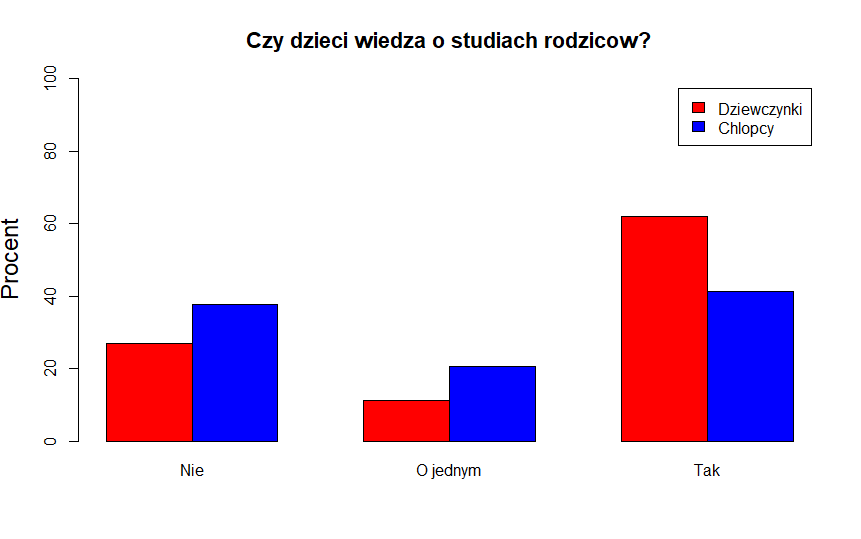
\includegraphics[width=0.5\textwidth]{1.png}
	\caption{Graf dotyczący wiedzy dzieci o studiach rodziców.}
	\label{fig:studies_knowledge}
\end{figure}
\begin{figure}
	\centering
	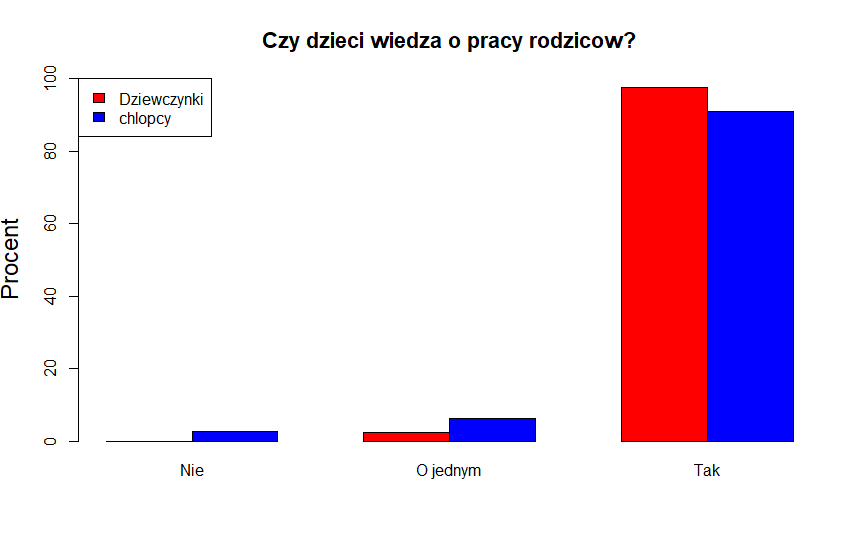
\includegraphics[width=0.5\textwidth]{2.png}
	\caption{Graf dotyczący wiedzy dzieci o pracy rodziców.}
	\label{fig:work_knowledge}
\end{figure}

Jak widać na załączonych rysunkach (ref. Rysunek~\ref{fig:studies_knowledge} oraz Rysunek~\ref{fig:work_knowledge}) dziewczynki mają lepszą wiedzę o rodzicach. Większa wiedza dziewczynek o studiach rodziców została potwierdzona testem Wilcoxona. Dodatkowo okazuje się, że dzieci więcej wiedzą o pracy rodziców, niż o ich studiach.

\subsection{Jaki jest wpływ otoczenia dziecka na oceny?}
Kolejną z rzeczy, które chcieliśmy sprawdzić była zależność między otoczeniem dziecka, a jego ocenami. W związku z tym chcieliśmy sprawdzić zależność między liczbą książek, studiami lub dopingiem rodziców. W tym celu policzyliśmy dla każdego dziecka średnią ocen.

\begin{figure}
	\centering
	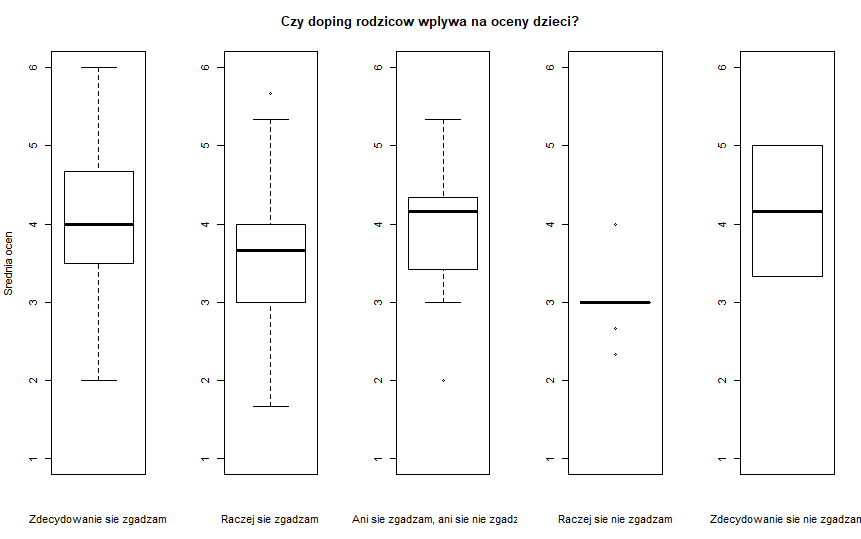
\includegraphics[width=0.5\textwidth]{3.png}
	\caption{Graf dotyczący zależności między dopingiem rodziców a  średnią ocen.}
	\label{fig:doping_oceny}
\end{figure}

Jak widać na załączonym grafie (ref. Rysunek~\ref{fig:doping_oceny}), doping rodziców zdaje się nie mieć wpływu na oceny uczniów. Niestety może to być związane z różnym rozumieniem pytania przez dzieci.

\begin{figure}
	\centering
	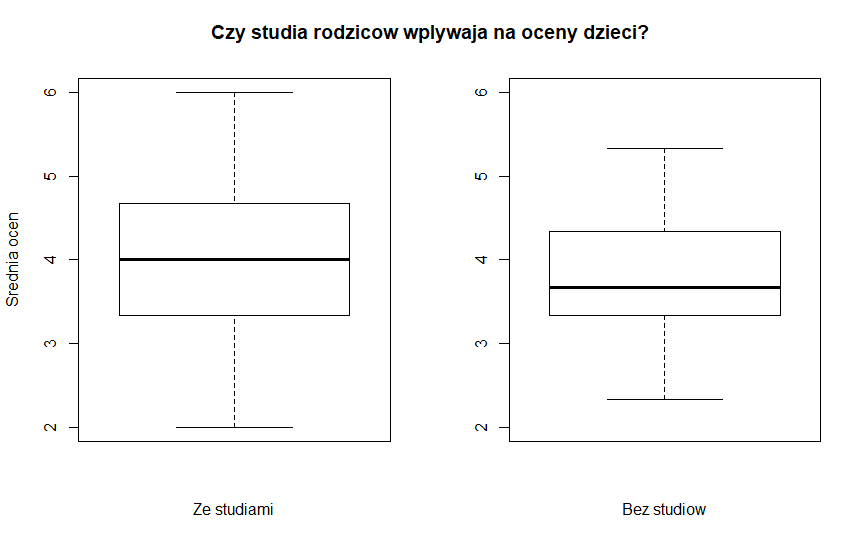
\includegraphics[width=0.5\textwidth]{4.png}
	\caption{Graf dotyczący zależności między studiami rodziców a średnią ocen.}
	\label{fig:studia_oceny}
\end{figure}

Studia rodziców zdają się mieć trochę większy wpływ na wyniki dzieci (ref. Rysunek~\ref{fig:studia_oceny}). Dzieci, których rodzice ukończyli studia i dzieci o tym wiedzą mają średnio lepsze wyniki w nauce, jednak statystyczna istotność tego faktu jest wątpliwa (p-value około 0.08).

\begin{figure}
	\centering
	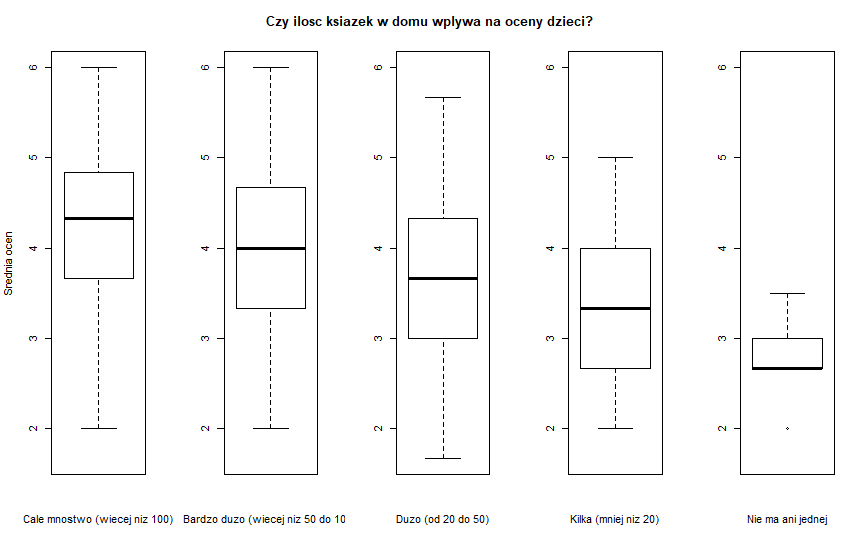
\includegraphics[width=0.5\textwidth]{5.png}
	\caption{Graf dotyczący zależności między liczbą książek w domu a średnią ocen.}
	\label{fig:ksiazki_oceny}
\end{figure}

Najlepsze efekty dało porównanie liczby książek w domu ze średnią (ref. Rysunek~\ref{fig:ksiazki_oceny}). Wyraźnie lepsze wyniki osiągają dzieci, w których otoczeniu znajduje się wiele książek. Jeśli w otoczeniu dziecka znajduje się przynajmniej 50 książek, to przeciętnie średnia ocen dziecka jest wyższa niż 4.0, co jest naprawdę bardzo dobrym wynikiem. Natomiast gdy nie ma żadnej książki, średnia spada poniżej 3.0. Jasno z tego wynika, że książki wpływają pozytywnie na rozwój dziecka.

\subsection{Czy jest zależność między kapitałem naukowym a ocenami?}
W ramach kolejnego zadania, chcieliśmy sprawdzić zależność między obliczonym kapitałem naukowym, a studiami rodziców i ocenami dzieci, jako że okazały się byc one najbardziej miarodajne.

\begin{figure}
	\centering
	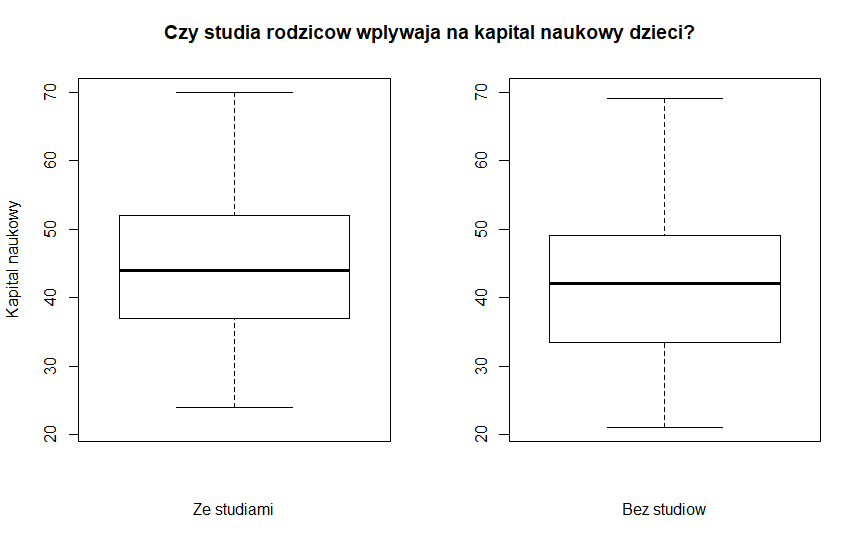
\includegraphics[width=0.5\textwidth]{6.png}
	\caption{Graf dotyczący zależności między studiami rodziców a kapitałem naukowym.}
	\label{fig:studia_kapital}
\end{figure}
\begin{figure}
	\centering
	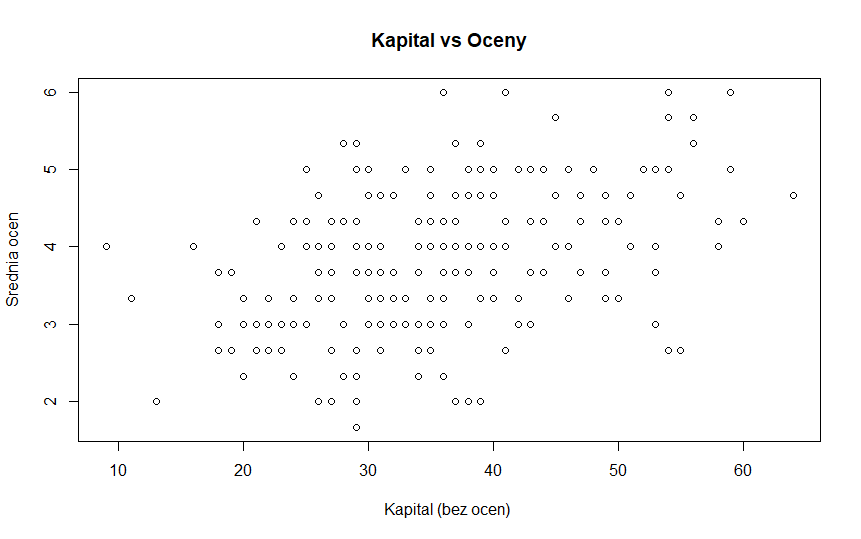
\includegraphics[width=0.5\textwidth]{7.png}
	\caption{Graf dotyczący zależności między ocenami a kapitałem naukowym z odliczonymi ocenami.}
	\label{fig:oceny_kapital}
\end{figure}

Wzięcie pod uwagę kapitału naukowego (ref. Rysunek~\ref{fig:studia_kapital}) zamiast ocen (ref. Rysunek~\ref{fig:studia_oceny}) dało bardziej zrównane wyniki. Co może świadczyć o niedokładności kapitału naukowego lub o braku zależności między ocenami a studiami rodziców.

Dość ładną natomiast okazała się zależność między ocenami, a kapitałem naukowym liczonym bez ocen (ref. Rysunek~\ref{fig:oceny_kapital}). Widać wyraźnie, że jest niezerowa korelacja. Sugeruje ona, że kapitał naukowy jest dość dobrym przybliżeniem potencjału dziecka.

\subsection{Czy istnieje zależność między typem zawodu, a ocenami?}
Wiele z danych, w tym na przykład zawody, zawierało literówki, bądź też bardzo różne formy opisu tego samego. W celu przefiltrowania danych pogrupowaliśmy zawody na związane z konkretnymi przedmiotami: Matematyką, Polskim i Przyrodą.
Chcieliśmy to także powiązać z ocenami z konkretnych przedmiotów. W tym celu pogrupowaliśmy oceny wedle przedmiotów by zobaczyć czy istnieje jakaś zależność.

\begin{figure}
	\centering
	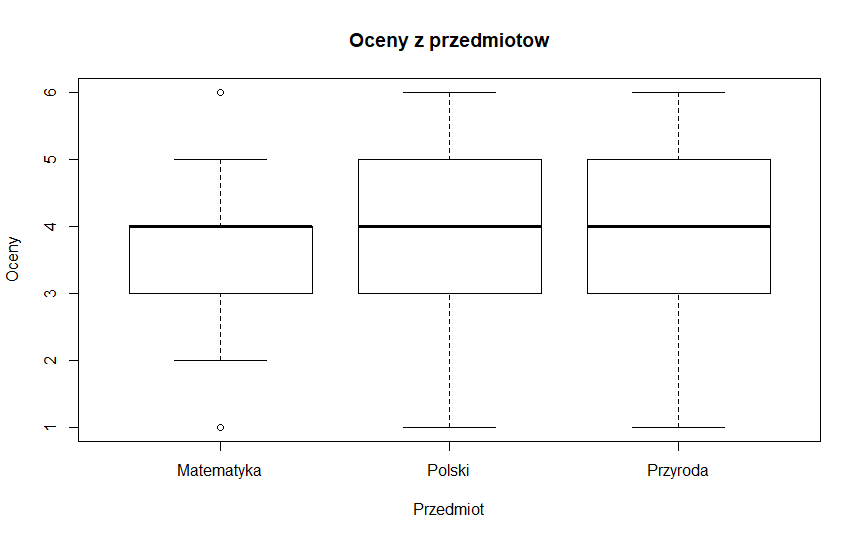
\includegraphics[width=0.5\textwidth]{8.png}
	\caption{Graf dotyczący ocen z konkretnych przedmiotów.}
	\label{fig:oceny}
\end{figure}

Jak widać na załączonym boxplocie (ref. Rysunek~\ref{fig:oceny}) oceny są bardzo wyrównane, choć matematyka zdaje się ogółem sprawiać więcej problemów.

Do przetwarzania ocen wykorzystaliśmy tylko oceny dzieci, których rodzice mieli zawód związany z Matematyką, Polskim i Przyrodą, natomiast odrzuciliśmy Inne i NA. Stworzyliśmy trzy grupy wedle przedmiotów i w nich podzieliliśmy dane na związane z przedmiotem (uczeń miał rodzica związanego z przedmiotem gdy przynajmniej jeden rodzic pracował \"w przedmiocie\"), bądź też nie. Wewnątrz tych podgrup wyliczyliśmy średnią ocen i porównaliśmy.

\begin{figure}
	\centering
	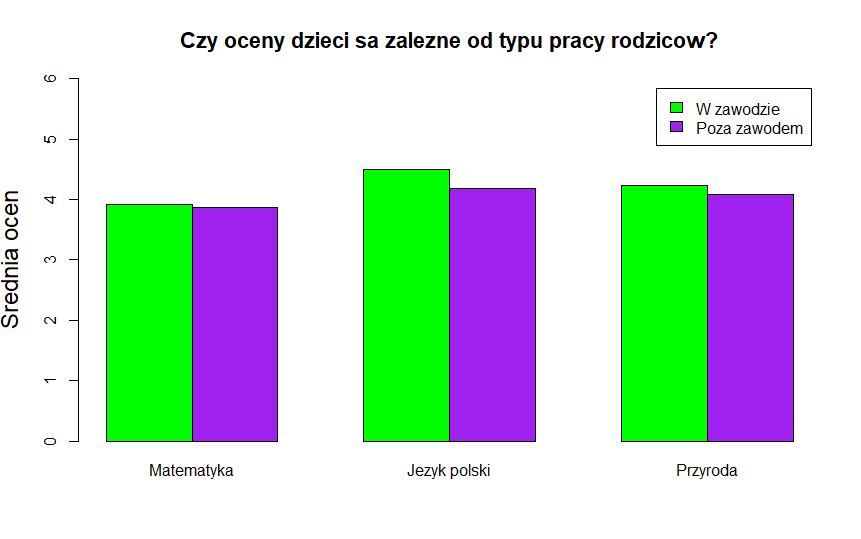
\includegraphics[width=0.5\textwidth]{9.png}
	\caption{Graf dotyczący zależności między pracą rodziców a oceną z danego przedmiotu.}
	\label{fig:oceny_praca}
\end{figure}

Jak widać (ref. Rysunek~\ref{fig:oceny_praca}), uczniowie najwięcej mogą zyskać, gdy praca ich rodziców jest powiązana z językiem polskim - różnica ocen między dziećmi osób niezwiązanych z polskim była największa. Zaskakująco najmniejsza była związana z matematyką.

\begin{figure}
	\centering
	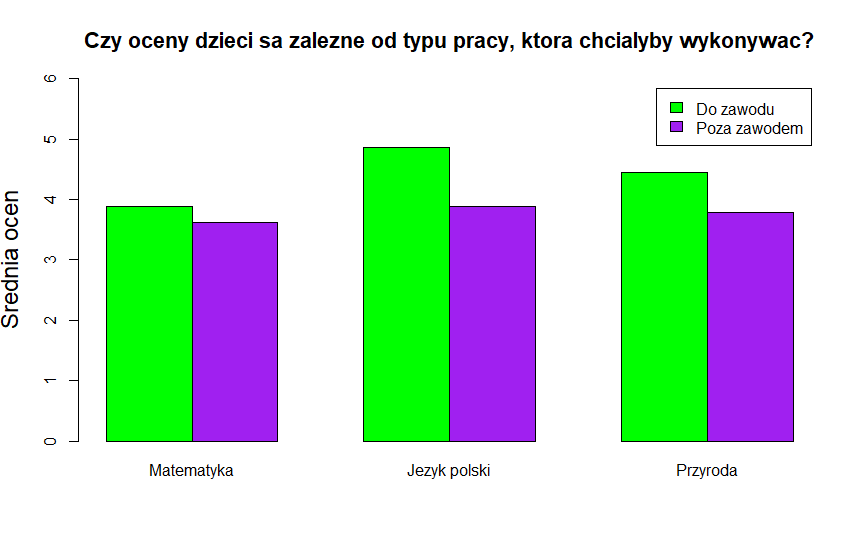
\includegraphics[width=0.5\textwidth]{10.png}
	\caption{Graf dotyczący zależności między wymarzoną pracą a oceną z danego przedmiotu.}
	\label{fig:oceny_wymarzona}
\end{figure}

Bardzo podobne wyniki osiągnęliśmy przy porównaniu ocen z wymarzoną pracą (ref. Rysunek~\ref{fig:oceny_wymarzona}). W tym przypadku jednak była większa różnica między ocenami dzieci "Do zawodu", a ocenami "Poza zawodem". Uznaliśmy, że może to wynikać z tego, że przedmiot typu matematyka jest uznawany za bardziej ustruktyruzowany, a co za tym idzie powtarzalny, w przeciwieństwie do polskiego, który jest bardziej oparty na kreatywności, której nie da się wpisać w schemat.

\subsection{Czy istnieje jakiś podział dzieci na grupy wedle ocen i ilości książek?}

Kolejnym zadaniem związanym z Ankietą było sprawdzenie czy korzystając z klasteryzacji jesteśmy w stanie wyróżnić jakieś grupy opierając się na wynikach uczniów i ilości książek w domu.

W tym celu wyszczególniliśmy dwa zbiory danych. W każdym znajdowała się średnia ocen dzieci i ilość książek, natomiast w jednym dodaliśmy także oceny do przetwarzania przez algorytm.

Najpierw musieliśmy się dowiedzieć, na ile klastrów powinniśmy podzielić nasz zbiór. Skorzystaliśmy z metody kolana by to ustalić (ref. Rysunek~\ref{fig:kolano_jeden} i Rysunek~\ref{fig:kolano_dwa}).

\begin{figure}
	\centering
	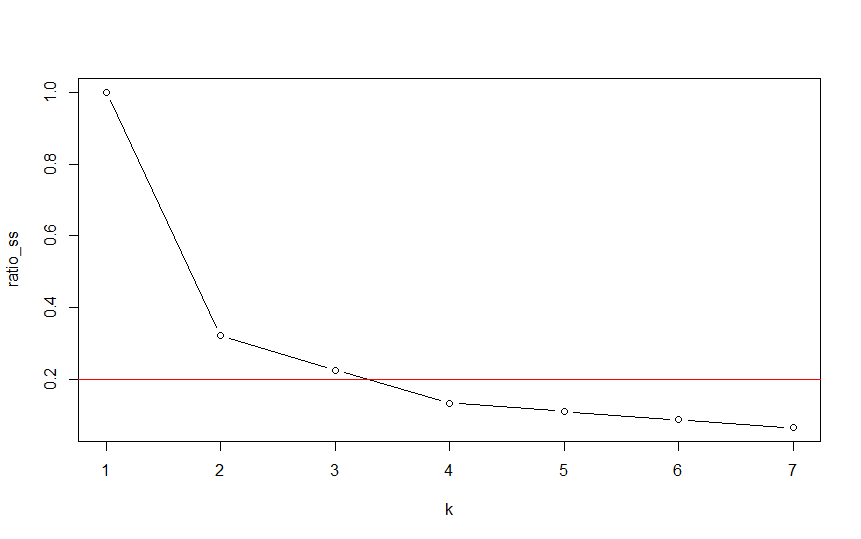
\includegraphics[width=0.5\textwidth]{11.png}
	\caption{Graf dotyczący ilości klastrów (średnia z ocenami).}
	\label{fig:kolano_jeden}
\end{figure}
\begin{figure}
	\centering
	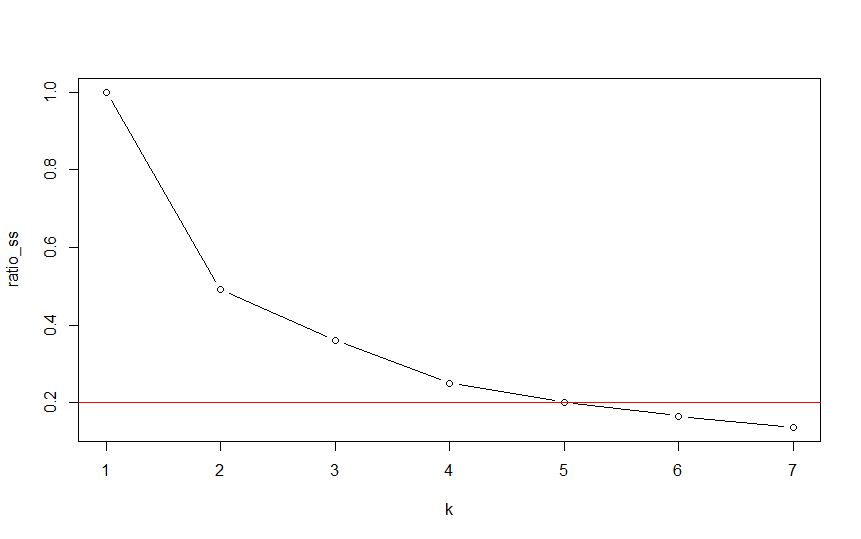
\includegraphics[width=0.5\textwidth]{12.png}
	\caption{Graf dotyczący ilości klastrów (tylko średnia).}
	\label{fig:kolano_dwa}
\end{figure}

Następnie porównaliśmy to z dendrogramami dla danych (ref. Rysunek~\ref{fig:dendrogramam_jeden} i Rysunek~\ref{fig:dendrogramam_dwa}). Niestety nie byliśmy w stanie określić jaka byłaby poprawna ilość klastrów, dlatego skorzystaliśmy z danych wyliczonych wcześniej.

\begin{figure}
	\centering
	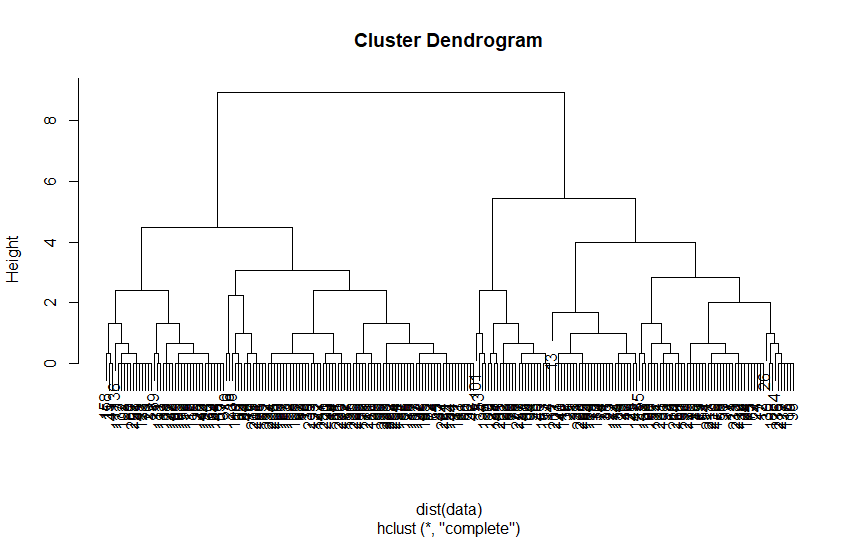
\includegraphics[width=0.5\textwidth]{13.png}
	\caption{Dendrogram (średnia z ocenami).}
	\label{fig:dendrogramam_jeden}
\end{figure}
\begin{figure}
	\centering
	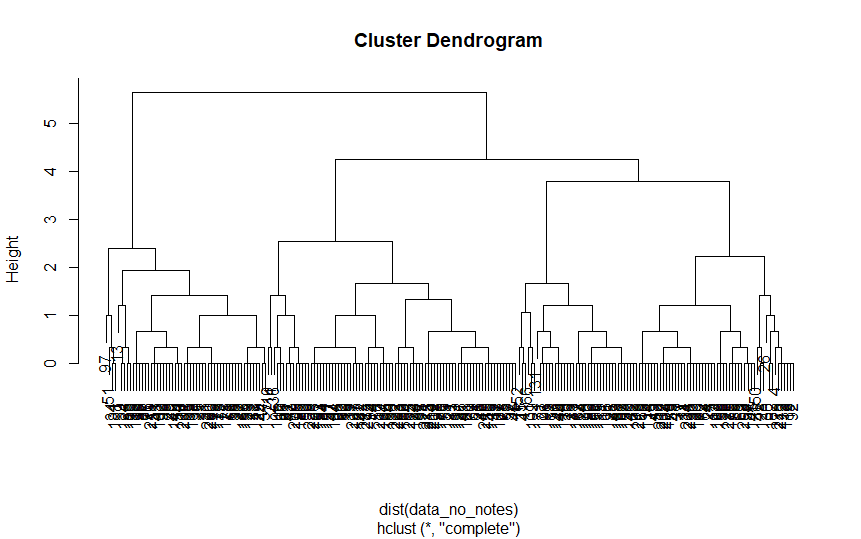
\includegraphics[width=0.5\textwidth]{14.png}
	\caption{Dendrogram (tylko średnia).}
	\label{fig:dendrogramam_dwa}
\end{figure}

Następnie korzystając z klastryzacji hierarchicznej otrzymaliśmy następujące wyniki (ref. Rysunek~\ref{fig:klaster}). Zdecydowaliśmy się na klasteryzację hierarchiczną, ponieważ jest ona lepsza dla stosunkowo małych zbiorów, a także w porównaniu do k-means jest bardziej dokładna.

\begin{figure}
	\centering
	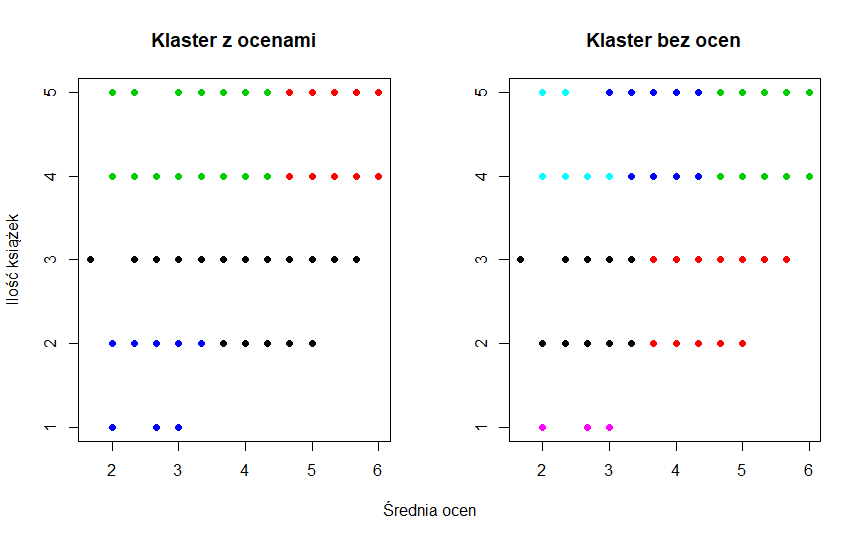
\includegraphics[width=0.5\textwidth]{15.png}
	\caption{Klater oceny i książki.}
	\label{fig:klaster}
\end{figure}

Z zadowoleniem znaleźliśmy potwierdzenie (ref. Rysunek~\ref{fig:klaster}) naszych obserwacji dotyczących istnienia pozytywnej zależności między ilością książek znajdujących się w domu, a ocenami (ref. Rysunek~\ref{fig:ksiazki_oceny}). Za korzystną uznaliśmy także zbieżność grup stworzonych poprzez dodanie ocen do jednej z grup - klaster okazał się być dzięki temu bardziej szczegółowy.


\section{Charakterystyka sposobu zwiedzania przez dzieci}
\subsection{Liczba odwiedzeń eksponatów w zależności od płci}
Na rysunku \ref{odwiedziny_plcie} przedstawiona jest zależność liczby odwiedzonych eksponatów od płci.
\begin{figure}[H]
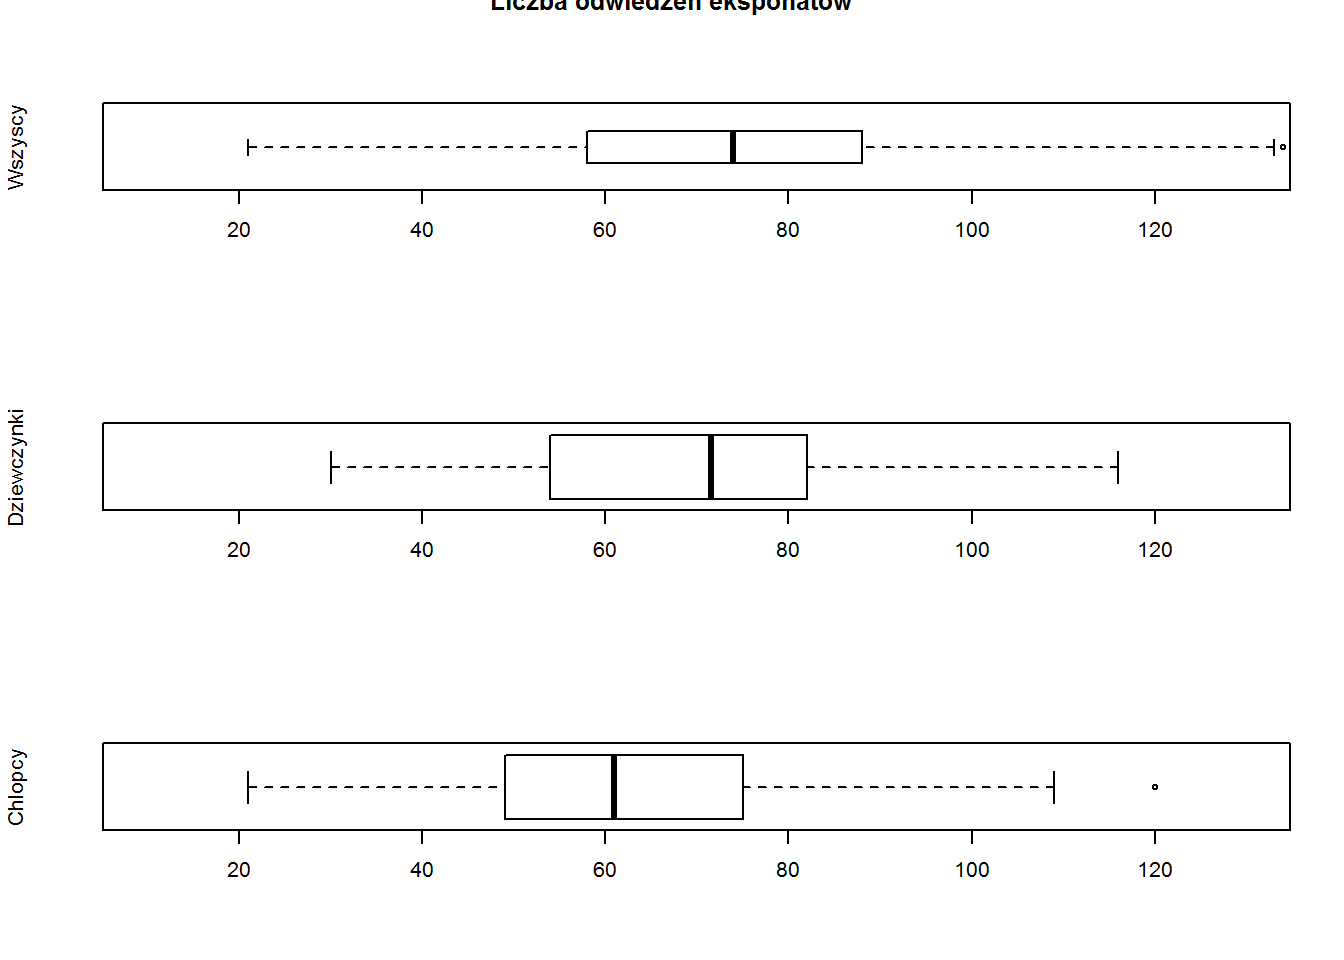
\includegraphics[width=0.48\textwidth]{odwiedziny_plcie.png}
\caption{Liczba odwiedzeń eksponatów w zależności od płci}
\label{odwiedziny_plcie}
\end{figure}
Pierwszy z wykresów przedstawiający odwiedziny wszystkich dzieci zawiera dane o wszystkich dzieciach, a dwa następne jedynie o tych, które wypełniały ankietę -- wskazuje to na istotne braki w danych.

\subsection{Liczebności grupek}
Na 204 dzieci zaobserwowano 3, które cały czas znajdowały się w jakiejś grupce i 3, które cały czas zwiedzały same. Pozostałe 198 część eksponatów odwiedziło w grupce, a część samemu.

Wykres \ref{grupki_liczba_eksponatow} przedstawia liczbę eksponatów zwiedzonych przez grupki różnych wielkości. Samotne zwiedzanie jest częstsze niż w grupce o jakiejkolwiek innej liczności, jednak zwiedzanie w grupce (dowolnej wielkości) jest częstsze niż samemu.

\begin{figure}[H]
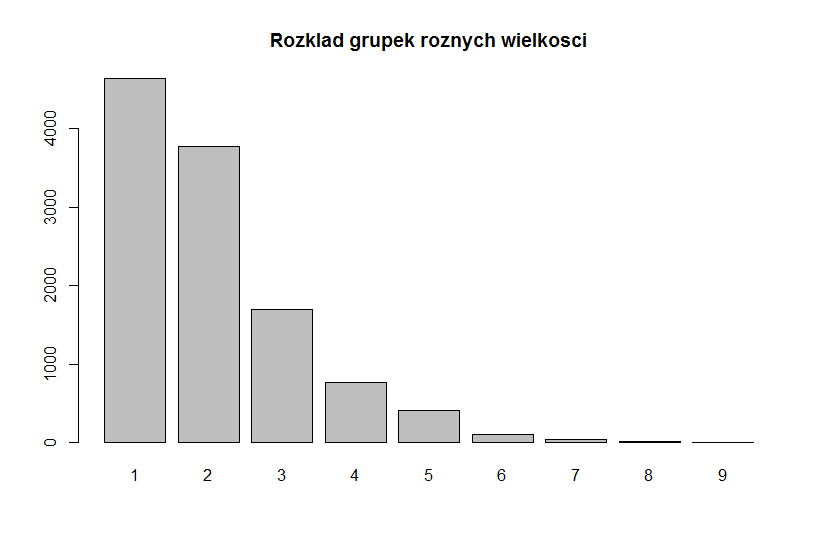
\includegraphics[width=0.48\textwidth]{grupki_liczba_eksponatow.png}
\caption{Liczba grupek w zależności od płci dzieci}
\label{grupki_plec}
\end{figure}

\subsection{Liczba odwiedzonych eksponatów w grupkach}
Tabela \ref{top_grupki1} przedstawia 10 grupek, które odwiedziły najwięcej eksponatów. Wystąpiły tam wyłącznie grupki 1- i 2-osobowe. Wynika to prawdopodobnie z faktu, że trudno, żeby większe grupki nie rozdzieliły się przez tak długi czas.
\begin{table}[H]
\caption{10 grupek o największej liczbie odwiedzonych eksponatów}
\label{top_grupki1}
\centering
\begin{tabular}{|c|r|r|}
\hline
 & \textbf{Liczba odwiedzonych eksponatów} & \textbf{Liczność grupki} \\
\hline
 1  &  101 & 1 \\
 2  &   90 & 2 \\
 3  &   86 & 2 \\
 4  &   84 & 2 \\
 5  &   82 & 1 \\
 6  &   80 & 2 \\
 7  &   78 & 2 \\
 8  &   77 & 1 \\
 9  &   72 & 2 \\
 10 &   70 & 1 \\
\hline
\end{tabular}
\end{table}

Kolejnym podejściem do tematu jest przyjrzenie się wyłącznie grupkom co najmniej 2 osobowym i tylko takim, dla których dało się sprawdzić płeć wszystkich dzieci. W tabeli \ref{top_grupki2} zostały wprowadzone te ograniczenia. Można zauważyć, że aż 8 z 10 najtrwalszych grupek składa się wyłącznie z dziewczyn. To sugeruje, że chłopcy częściej zmieniają towarzyszy podczas zwiedzania.

\begin{table}[H]
\caption{10 grupek o największej liczbie odwiedzonych eksponatów (dane przefiltrowane)}
\label{top_grupki2}
\centering
\begin{tabular}{|c|r|r|r|}
\hline
 & \textbf{Liczba odwiedzonych eksponatów} & \textbf{Liczność grupki}  & \textbf{Płeć grupki} \\
\hline
 1  & 78 & 2 & dziewczęca \\
 2  & 62 & 3 & dziewczęca \\
 3  & 60 & 2 & dziewczęca \\
 4  & 59 & 2 & dziewczęca \\
 5  & 57 & 2 & dziewczęca \\
 6  & 56 & 2 & mieszana  \\
 7  & 54 & 3 & dziewczęca \\
 8  & 50 & 2 & dziewczęca \\
 9  & 45 & 2 & chłopięca  \\
 10 & 44 & 2 & dziewczęca \\
\hline
\end{tabular}
\end{table}

Zależność tę można pokazać korzystając z całego zestawu danych. Wykres \ref{grupki_d_c_liczba_eksponatow} obrazuje liczby odwiedzonych eksponatów dla grupek, które odwiedziły co najmniej 5 eksponatów (większość grupek odwiedziło niewiele eksponatów w stałym składzie, więc uwzględnienie ich ukrywało zależność występującą dla trwalszych grupek). Można zauważyć, że o ile mediana jest podobna dla chłopców i dziewczynek, to w przypadku górnego kwartyla i decyla 9/10 są one znacznie większe dla dziewczynek.

\begin{figure}[H]
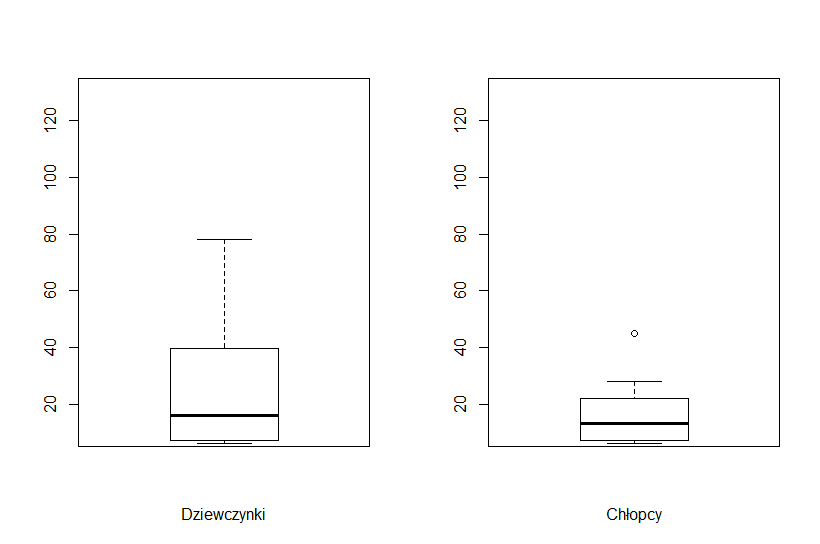
\includegraphics[width=0.48\textwidth]{grupki_d_c_liczba_eksponatow.png}
\caption{Wykres pudełkowy liczby eksponatów odwiedzonych przez grupki dziewczęce i chłopięce}
\label{grupki_d_c_liczba_eksponatow}
\end{figure}


\subsection{Rozkład grupek ze względu na płeć}
Wykres \ref{grupki_plec} przedstawia podział grupek na 3 kategorie: wyłącznie dziewczęce (239), wyłącznie chłopięce (271) i mieszane (294). Liczba grupek każdego z tych rodzajów jest zbliżona, jednak najwięcej jest grupek mieszanych.

\begin{figure}[H]
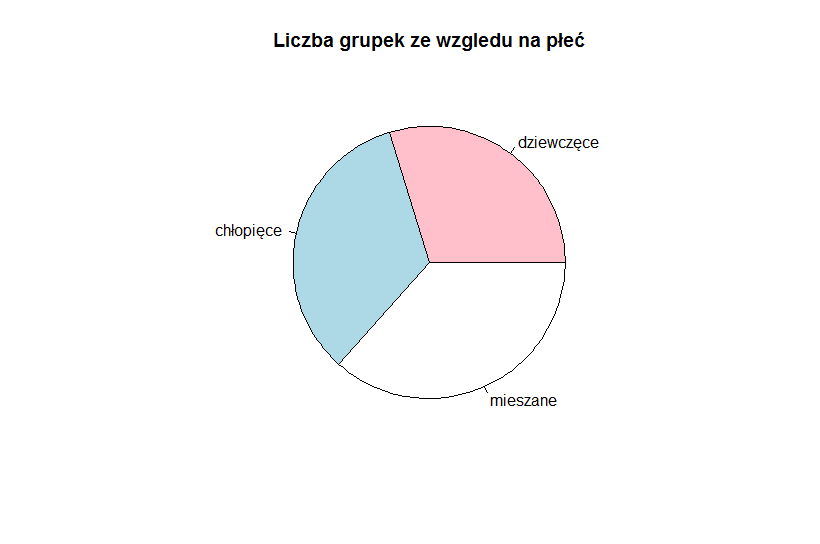
\includegraphics[width=0.48\textwidth]{grupki_plec.png}
\caption{Liczba grupek w zależności od płci dzieci}
\label{grupki_plec}
\end{figure}

\subsection{Klasteryzacja dzieci ze względu na styl zwiedzania}
W celu wyznaczenia klastrów, reprezentujących style zwiedzania zostały najpierw wybrane dwie cechy, opisujące zwiedzanie - liczba odwiedzonych eksponatów i średni czas przy eksponacie. Wybór liczby klastrów przebiegał dwustopniowo. Najpierw możliwe liczby klastrów zostały wybrane na podstawie wykresu \ref{style_zwiedzania_elbow}.

\begin{figure}[H]
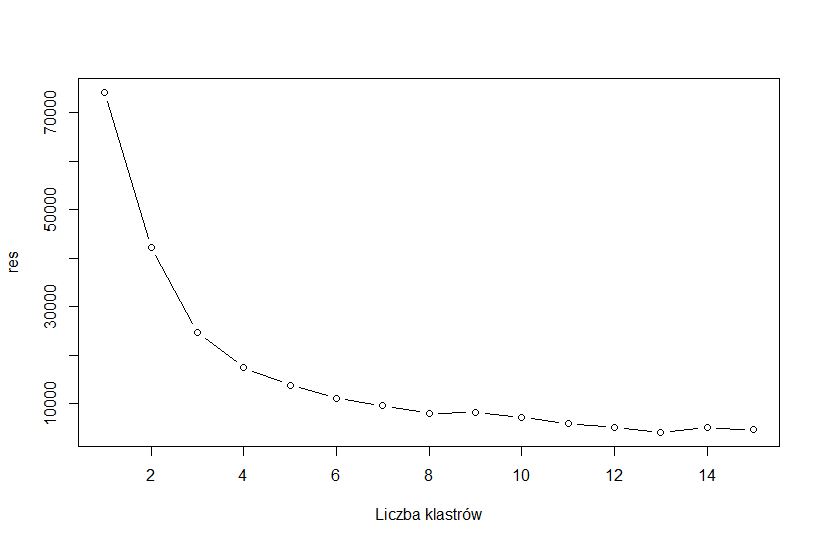
\includegraphics[width=0.48\textwidth]{style_zwiedzania_elbow.png}
\caption{Wykres łokciowy}
\label{style_zwiedzania_elbow}
\end{figure}

Wydaje się, że najkorzystniejszy byłby wybór 4 klastrów, jednak po sprawdzeniu efektów podziału na 3, 4 i 5 klastrów za najbardziej obiecującą została uznana ostatnia opcja - tylko w tej wersji wyodrębnił się klaster zawierający dzieci, które zwiedziły niewiele eksponatów przy każdym spędzając stosunkowo krótki czas.

\begin{figure}[H]
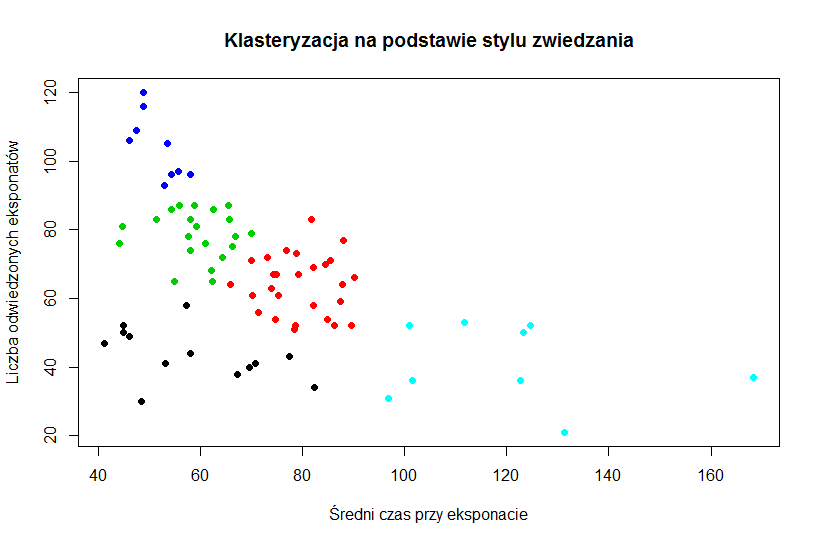
\includegraphics[width=0.48\textwidth]{style_zwiedzania.png}
\caption{Klasteryzacja względem liczby odwiedzonych eksponatów i średniego czasu przy eksponacie}
\label{style_zwiedzania}
\end{figure}

Można zauważyć, że prawy górny róg wykresu jest pusty. Jest to oczekiwany wynik - czas trwania wizyt w CNK był za krótki, żeby jednocześnie obejrzeć wiele eksponatów i każdemu poświęcić dużo czasu.

Dla uzyskanych klastrów została policzona średnia dwóch parametrów: średniej (rysunek \ref{srednie_w_klastrach}) i kapitału naukowego bez ocen (rysunek \ref{kapital_w_klastrach}).

\begin{figure}[H]
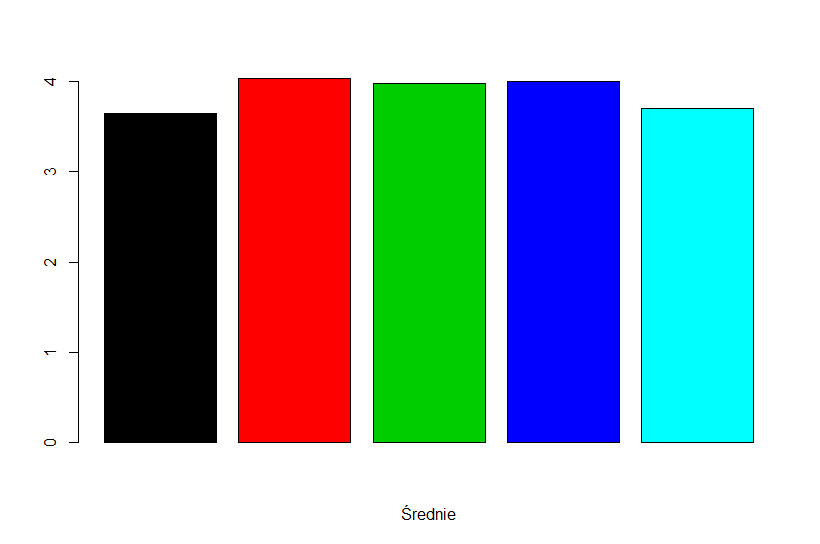
\includegraphics[width=0.48\textwidth]{srednie_w_klastrach.png}
\caption{Średnia ocen w klastrach}
\label{srednie_w_klastrach}
\end{figure}

\begin{figure}[H]
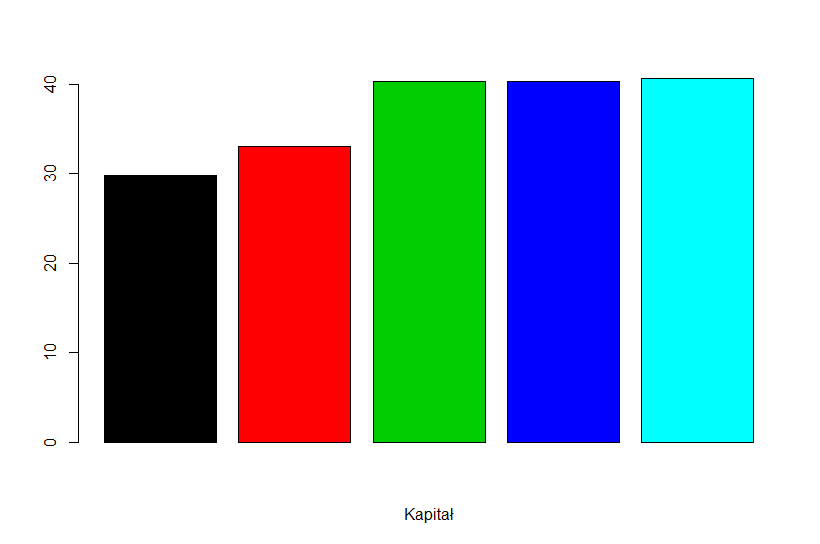
\includegraphics[width=0.48\textwidth]{kapital_w_klastrach.png}
\caption{Kapitał naukowy w klastrach}
\label{kapital_w_klastrach}
\end{figure}

W obu porównaniach najgorzej wypada grupa dzieci, które były przy niewielu eksponatach, średnio dość krótko przy każdym.
Dodatkowo średnio słabsze oceny mają dzieci, których średni czas przy eksponatach jest wysoki.
Z kolei niższym kapitałem naukowym wykazują się osoby, których średni czas przy eksponacie jest raczej duży, a liczba odwiedzonych eksponatów średnia. Równocześnie dzieci z tej grupy osiągają dobre wyniki w szkole. 

\subsection{Wielokrotne odwiedzanie eksponatów}
Średnia liczba odwiedzeń eksponatu przez dziecko, które już go odwiedziło, wynosi:
\begin{itemize}
\item Dla wszystkich dzieci: 1.228,
\item Dla 20 dzieci z najwyższym kapitałem naukowym: 1.167,
\item Dla 20 dzieci z najniższym kapitałem naukowym: 1.234.
\end{itemize}
Rangowy test Wilcoxona potwierdza, że różnica między dziećmi z najwyższym kapitałem, a pozostałymi, jest statystycznie istotna -- rzadziej podchodzą więcej niż raz do tego samego eksponatu.
\subsection{Liczba unikalnych odwiedzeń eksponatów}
Średnia liczba unikalnych odwiedzeń eksponatów przez dzieci to:
\begin{itemize}
\item Dla wszystkich dzieci: 54.1,
\item Dla 20 dzieci z najwyższym kapitałem naukowym: 55.4,
\item Dla 20 dzieci z najniższym kapitałem naukowym: 49.4.
\end{itemize}
Ponieważ test Shapiro-Wilka nie odrzucił hipotezy o normalności rozkładu tych danych, w celu sprawdzenia statystycznej istotności różnic, zastosowany został t-test Studenta. Na jego podstawie różnice nie są istotne.
>>>>>>> cc3d1700110c3b52eca3cf3d39c3a5d1452e1394

\section{Analiza eksponatów}
Analiza eksponatów została wykonana na wystawach z kategorii 2, czyli z wyłączeniem wszystkich przerw, a także obiektów sklasyfikowanych jako ,,inne", czyli na przykład \textit{Majsterni}.
\subsection{Popularność galerii}
Rysunek \ref{galerie} przedstawia liczbę odwiedzeń eksponatów w poszczególnych galeriach -- w wersji nieprzetworzonej, a także znormalizowanej ze względu na liczbę eksponatów w galerii.
\begin{figure}[H]
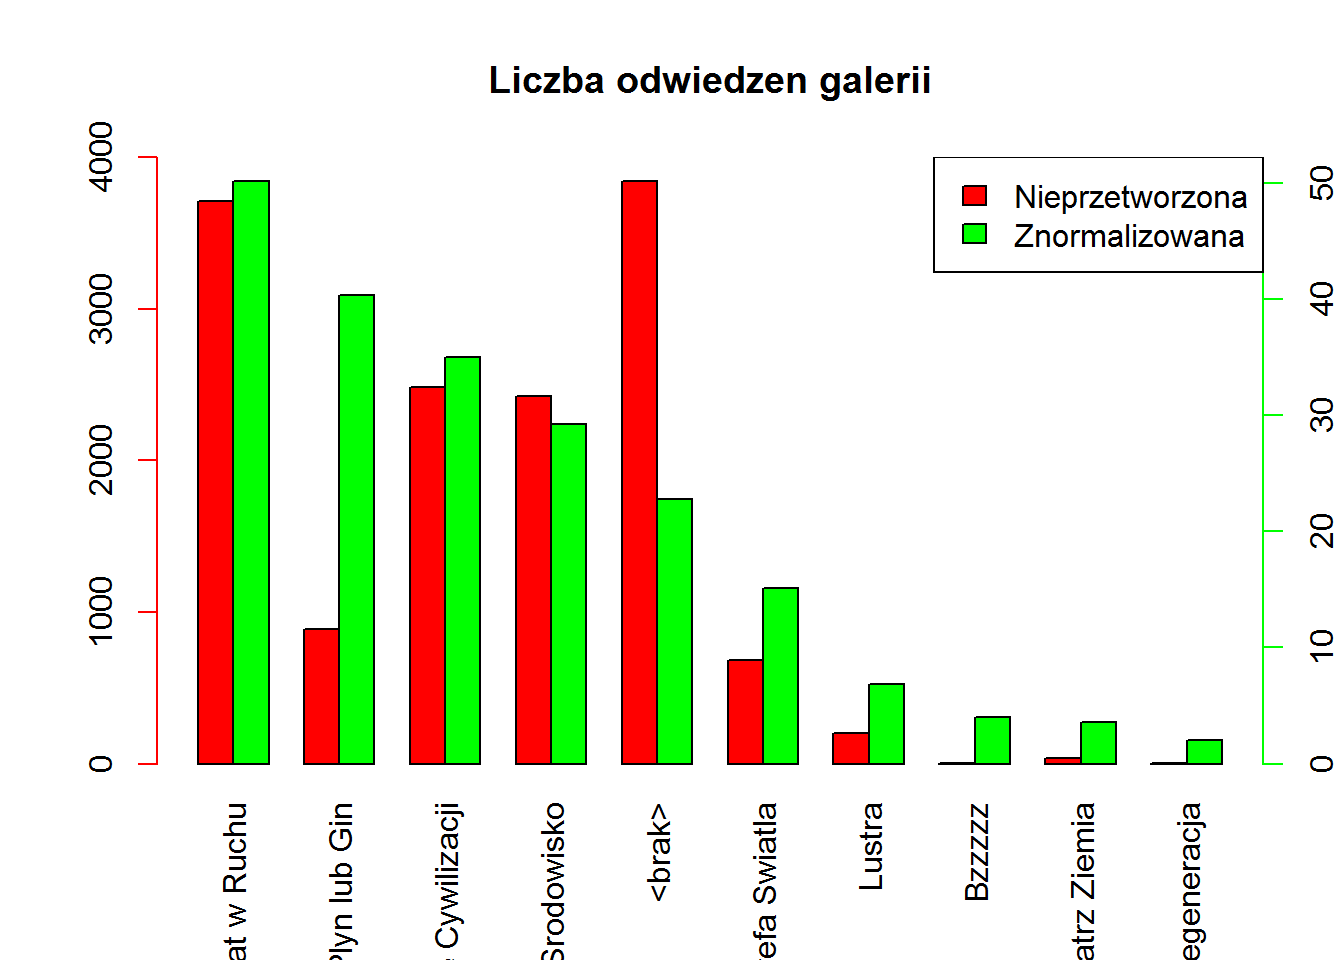
\includegraphics[width=0.48\textwidth]{galerie.png}
\caption{Liczba odwiedzeń poszczególnych galerii}
\label{galerie}
\end{figure}
Normalizacja nie jest w pełni dokładna, ponieważ liczone były jedynie te eksponaty, które zostały odwiedzone co najmniej raz (ze względu na brak kompletnej listy eksponatów) -- anomalie wynikające z tego są szczególnie widoczne w przypadku trzech ostatnich galerii, których liczba odwiedzeń była bardzo niewielka.
\subsection{Popularność eksponatów}
Tabela \ref{top_eksponaty} przedstawia listę najpopularniejszych eksponatów.
\begin{table}[H]
\caption{Najpopularniejsze eksponaty}
\label{top_eksponaty}
\centering
\begin{tabular}{|r|l|l|l|}
\hline
\textbf{Lp.} & \textbf{Eksponat} & \textbf{Galeria} & \textbf{Odwiedziny} \\
\hline
 1 &   ALARM NA STATKU  &     Plyn lub Gin     &         220 \\
 2 &   OKNO KOPERNIKA & Nowy Swiat w Ruchu    &          209 \\
 3 &   MYDLANA SCIANA & Nowy Swiat w Ruchu   &           113 \\
 4 &           CHOMIK  &           ---    &          111 \\
 5 &          TORNADO & Nowy Swiat w Ruchu    &          110 \\
 6 & DOMEK ZE SKRZYNIA  &           ---   &          108 \\
\hline
\end{tabular}
\end{table}
Jak widać, pierwzse dwa eksponaty cieszyły się szczególną popularnością. Dalsze badania wskazały, że najpopularniejsze eksponaty dla grupy 20 uczniów z największym kapitałem naukowym i dla grupy 20 dzieci z najmniejszym kapitałem pokrywały się. Wyjątkami, czyli eksponatami występującymi wśród 10 najpopularniejszych u jednej grupy, ale niewystępującymi wśród 20 najpopularniejszych u drugieej grupy, były:
\begin{itemize}
\item \textit{Wahadło Foucault} na 7. miejscu u dzieci z najwyższym kapitałem,
\item \textit{Silnik roślinny} na 10. miejscu u dzieci z najwyższym kapitałem,
\item \textit{I tłoki turkocą} na 6. miejscu u dzieci z najniższym kapitałem.
\end{itemize}
\subsection{Najpopularniejsze eksponaty w obrębie każdej galerii}
Tabela \ref{top_eksponaty_galerie} pokazuje najpopularniejszy eksponat w każdej galerii.

\begin{table}[H]
\caption{Najpopularniejsze eksponaty w obrębie każdej galerii}
\label{top_eksponaty_galerie}
\centering
\begin{tabular}{|r|l|l|l|}
\hline
\textbf{Lp.} & \textbf{Galeria} & \textbf{Eksponat} & \textbf{Odw.} \\
\hline

1  &          Plyn lub Gin &           ALARM NA STATKU &  220  \\
2  &    Nowy Swiat w Ruchu &            OKNO KOPERNIKA &              209  \\
3  &                ---    &                    CHOMIK &              111  \\
4  &  Korzenie Cywilizacji &            LASEROWA HARFA &               95  \\
5  & Czlowiek i Srodowisko & BIEGANIE (3,2,1\ldots START!) &               83  \\
6  &        Strefa Swiatla &        UKRYTA PERSPEKTYWA &               42  \\
7  &                Lustra &    ZWIERCIADLANY LABIRYNT &               30  \\
8  &          Patrz Ziemia &     ODBIORNIK SATELITARNY &                7  \\
9  &                Bzzzzz &                  OSWOJAKI &                4  \\
10 &           Regeneracja &      ROZPOZNAWANIE TWARZY &                2  \\
\hline
\end{tabular}
\end{table}
Zgodnie z intuicją, w rzadziej odwiedzanych galeriach (patrz rys. \ref{galerie}) również najpopularniejsze eksponaty otrzymały znacząco mniejszą liczbę odwiedzin.

\subsection{Najbardziej absorbujące eksponaty}
Przeprowadzona została analiza najbardziej absorbujących eksponatów, według następujących kryteriów:
\begin{itemize}
\item Średniego spędzonego czasu,
\item Średniego osiąganego poziomu eksploracji,
\item Frakcji dzieci, które przeczytały opis,
\item Frakcji dzieci, które rozmawiały z animatorem.
\end{itemize}
Dla każdego z tych kryteriów zostały znalezione wiodące eksponaty. Uwzględniane były jedynie eksponaty, które zostały odwiedzone ponad 10 razy, w celu odrzucenia anomalii spowodowanej bardzo małą próbką. Ponadto, znalezione zostały najlepsze według tych kryteriów eksponaty w obrębie każdej galerii, z wyłączeniem trzech najrzadziej odwiedzanych. Dla niektórych kryteriów dodatkowo powstały dodatkowe listy pomijające eksponaty nieposiadające galerii, ze względu na ich widoczną dominację.
\subsubsection{Średni spędzony czas}
Średni czas spędzony na pojedynczym eksponacie to 56.5 sekundy. Tabela \ref{top_czas} przedstawia eksponaty, przy których wizyty średnio zajmowały najwięcej czasu. Podany czas jest reprezentowany w sekundach.

\begin{table}[H]
\caption{Średni czas wizyty przy eksponacie}
\label{top_czas}
\centering
\begin{tabular}{|r|l|l|l|}
\hline
\textbf{Lp.} & \textbf{Eksponat} & \textbf{Galeria} & \textbf{Czas} \\
\hline
1  &         PRZEBUDOWA &                --- &  408.4    \\
2  &       MEMORY FLOOR &                --- &  275.7    \\
3  &             OCULUS &                --- &  256.2    \\
4  &    PIJANY KIEROWCA & Czlowiek i Srodowisko &  181.2    \\
5  &  POJEDYNEK UMYSLOW & Czlowiek i Srodowisko &  179.6    \\
6  & LABIRYNT PRZESZKOD & Czlowiek i Srodowisko &  167.3    \\
7  & KOSMICZNY SMIETNIK &    Nowy Swiat w Ruchu &  162.6    \\
8  &             SEKCJA &                --- &  157.4    \\
9  & AUKCJA HOLENDERSKA &  Korzenie Cywilizacji &  150.6    \\
10 &           ANATOMIA &                --- &  149.4    \\
\hline
\end{tabular}
\end{table}
Pierwsze trzy eksponaty istotnie wyróżniają się. Warto zauważyć, że są to eksponaty poza galeriami. Pozostałe siedem eksponatów ma już bardziej zbliżony średni czas wizyty.

W tabeli \ref{top_czas_g} wskazane są eksponaty o najdłuższym średnim czasie wizyty dla każdej galerii.
\begin{table}[H]
\caption{Średni czas wizyty przy eksponacie}
\label{top_czas_g}
\centering
\begin{tabular}{|r|l|p{3.4cm}|l|}
\hline
\textbf{Lp.} & \textbf{Galeria} & \textbf{Eksponat} & \textbf{Czas} \\
\hline
1 &                ---    &              PRZEBUDOWA    & 408.4 \\
2 & Czlowiek i Srodowisko &            PIJANY KIEROWCA & 181.2 \\
3 &  Korzenie Cywilizacji &         AUKCJA HOLENDERSKA & 150.6 \\
4 &                Lustra &               DUCH PEPPERA & 49.4 \\
5 &    Nowy Swiat w Ruchu &         KOSMICZNY SMIETNIK & 162.6 \\
6 &          Plyn lub Gin & ZJAZD DO TRATWY RATUNKOWEJ & 132.5 \\
7 &        Strefa Swiatla &              ZOLTE SWIATLO & 111.8 \\
\hline
\end{tabular}
\end{table}
Zgodnie z przewidywaniami, istotną grupą wśród najdłużej używanych eksponatów są wystawy w formie gier, tak jak \textit{Kosmiczny śmietnik}, czy \textit{Pijany kierowca}. Poza wcześniej wspomnianymi odstającymi obserwacjami spoza galerii, to zestawienie ujawniło, że eksponaty w galerii \textit{Lustra} są wykorzystywane bardzo krótko -- najdłuższy czas w tej galerii, 49.4 sekundy, to mniej, niż przeciętny czas spędzony przy eksponacie w obrębie całego centrum nauki. 
\subsubsection{Średni osiągnięty poziom eksploracji}
Ponieważ zdecydowaliśmy, że ,,bezmyślne" dotykanie eksponatu nie jest wyższym poziomem, niż patrzenie (a w wielu przypadkach można nawet stwierdzić, że to niższy poziom), pierwotna skala została zmodyfikowana -- 1 oznacza jedynie dotykanie lub jedynie patrzenie, 2 -- korzystanie, a 3 -- eksperymentowanie. Średni poziom w tej skali dla wszystkich eksponatów to 1.66. Warto zwrócić uwagę, że nie wszystkie eksponaty pozwalały na każdy poziom -- na niektóre można było tylko patrzeć, a w wielu nie były możliwe eksperymenty. Tabela \ref{top_zach} przedstawia najbardziej eksplorowane wystawy.
\begin{table}[H]
\caption{Średni poziom eksploracji}
\label{top_zach}
\centering
\begin{tabular}{|r|l|l|l|}
\hline
\textbf{Lp.} & \textbf{Eksponat} & \textbf{Galeria} & \textbf{Poziom} \\
\hline
1  &                DJ &             ---        &     2.08    \\
2  &      DUCH PEPPERA &             Lustra     &        2.00 \\
3  &   KOLOROWE CIENIE &     Strefa Swiatla     &        2.00 \\
4  &       PODUSZKOWCE &             ---        &     2.00    \\
5  &          RURA 900 &             ---        &     1.96    \\
6  &  PRZEWROTNA KULKA & Nowy Swiat w Ruchu     &        1.95 \\
7  &          RUROCIAG &             ---        &     1.95    \\
8  &            MOTORY &             ---        &     1.94    \\
9  &           NA FALI &             ---        &     1.92    \\
10 &          ANATOMIA &             ---        &     1.92    \\
\hline
\end{tabular}
\end{table}
Narzucającą się na pierwszy rzut oka obserwacją jest zdecydowana dominacja eksponatów spoza galerii -- sugeruje to, że zwykle są one bardziej interaktywne, niż pozostałe. Warto też zwrócić na eksponat \textit{Duch Peppera}: jest to eksponat z galerii \textit{Lustra}, przy którym dzieci spędzały najwięcej czasu (a jednocześnie poniżej przeciętnej) -- na podstawie powyższych informacji można wywnioskować, że po prostu ten eksponat nie wymagał dużo czasu, ponieważ trudno by było uwierzyć, żeby z jakiegokolwiek innego powodu dzieci spędzały go tak mało przy wyjątkowo absorbującym eksponacie.
Tabela \ref{top_zach_b} nie uwzględnia eksponatów bez galerii.
\begin{table}[H]
\caption{Średni poziom eksploracji}
\label{top_zach_b}
\centering
\begin{tabular}{|r|l|l|l|}
\hline
\textbf{Lp.} & \textbf{Eksponat} & \textbf{Galeria} & \textbf{Poziom} \\
\hline
1  &       DUCH PEPPERA &                Lustra & 2.00 \\
2  &    KOLOROWE CIENIE &        Strefa Swiatla & 2.00 \\
3  &   PRZEWROTNA KULKA &    Nowy Swiat w Ruchu & 1.95 \\
4  &     ORKIESTRA TUSZ &  Korzenie Cywilizacji & 1.89 \\
5  &        ZYWE SREBRO &    Nowy Swiat w Ruchu & 1.89 \\
6  &              DIETA & Czlowiek i Srodowisko & 1.88 \\
7  &   WAHADLO SWIETLNE &    Nowy Swiat w Ruchu & 1.88 \\
8  & MAGNETYCZNA CHMURA &    Nowy Swiat w Ruchu & 1.86 \\
9  &       WYSCIG LODZI &  Korzenie Cywilizacji & 1.82 \\
10 &      PRZESLUCHANIE &        Strefa Swiatla & 1.81 \\
\hline
\end{tabular}
\end{table}
W tym zestawieniu rozkład galerii jest znacznie bardziej równomierny.
Tabela \ref{top_zach_g} to zestawienie najbardziej eksplorowanych eksponatów w obrębie każdej galerii.

\begin{table}[H]
\caption{Średni poziom eksploracji}
\label{top_zach_g}
\centering
\begin{tabular}{|r|l|l|l|}
\hline
\textbf{Lp.} & \textbf{Galeria} & \textbf{Eksponat} & \textbf{Poziom} \\
\hline
1 &                ---    &            DJ    &  2.08	\\
2 & Czlowiek i Srodowisko &            DIETA &     1.88	\\
3 &  Korzenie Cywilizacji &   ORKIESTRA TUSZ &     1.89	\\
4 &                Lustra &     DUCH PEPPERA &                    2.00	\\
5 &    Nowy Swiat w Ruchu & PRZEWROTNA KULKA &     1.95	\\
6 &          Plyn lub Gin &   SRUBA NAPEDOWA &     1.56	\\
7 &        Strefa Swiatla &  KOLOROWE CIENIE &                    2.00	\\
\hline
\end{tabular}
\end{table}
W powyższym zestawieniu warto zwrócić uwagę, że najbardziej eksplorowana wystawa z galerii \textit{Płyń lub giń} ma poziom 1.56, czyli niższy, niż średni w obrębie całej galerii -- można wnioskować, że to w tej galerii dzieci najczęściej bezmyślnie się bawią lub tylko obserwują. 

\subsubsection{Frakcja dzieci, które przeczytały opis}
Opis był czytany przez dzieci w 10\% przypadków. Należy zauważyć, że przeczytanie opisu raczej nie implikuje, że eksponat jest ciekawszy niż inne -- dzieci najprawdopodobniej robią to w ostateczności, jeśli bez tego nie mogą zrozumieć eksponatu. Z drugiej strony, jeśli wystawa nie wydaje im się ciekawa i jej nie rozumieją, dużo dzieci zamiast przeczytania opisu może się zniechęcić i odejść -- tak więc możliwym jest, że eksponaty, przy których dzieci najczęściej czytały opis, były relatywnie skomplikowane, ale jednocześnie ciekawe.
Tabela \ref{top_opis} przedstawia wystawy, przy których dzieci najczęściej sięgały po opis.
\begin{table}[H]
\caption{Frakcja dzieci, które przeczytały opis}
\label{top_opis}
\centering
\begin{tabular}{|r|p{3.3cm}|l|l|}
\hline
\textbf{Lp.} & \textbf{Eksponat} & \textbf{Galeria} & \textbf{Opis} \\
\hline
1  &                  DUCH PEPPERA &                Lustra & 0.58 \\
2  &                 RADIO W GEBIE &    Nowy Swiat w Ruchu & 0.39 \\
3  &              FIGURY LISSAJOUS &    Nowy Swiat w Ruchu & 0.36 \\
4  &             OCZY Z TYLU GLOWY &                Lustra & 0.36 \\
5  & CZESCI ZAMIENNE DLA CZLOWIEKA & Czlowiek i Srodowisko & 0.36 \\
6  &                  PALACY CHLOD & Czlowiek i Srodowisko & 0.35 \\
7  &               CHCA BYC PIEKNI & Czlowiek i Srodowisko & 0.33 \\
8  &        PO GLOSIE CIE POZNAJA? & Czlowiek i Srodowisko & 0.33 \\
9  &       PRZENOSNY MOST LEONARDA &  Korzenie Cywilizacji & 0.33 \\
10 &                SKACZACA KULKA &    Nowy Swiat w Ruchu & 0.33 \\
\hline
\end{tabular}
\end{table}
Tylko przy jednej wystawie ponad połowa zwiedzających dzieci przeczytała opis. Wystąpiły aż dwa eksponaty z galerii \textit{Lustra} (w której było niewiele odwiedzonych eksponatów), w której maksymalny czas był mniejszy, niż średni czas z całego centrum nauki -- potwierdza to tezę, że wcześniejsza obserwacja wynikała jedynie z charakteru eksponatów, a nie braku zainteresowania. Ponadto, w zestawieniu nie wystąpił ani jeden eksponat bez galerii.
Tabela \ref{top_opis_g} to zestawienie eksponatów, które najczęściej wymagały czytania opisu, dla każdej galerii.
\begin{table}[H]
\caption{Frakcja dzieci, które przeczytały opis}
\label{top_opis_g}
\centering
\begin{tabular}{|r|l|p{3.3cm}|l|}
\hline
\textbf{Lp.} & \textbf{Galeria} & \textbf{Eksponat} & \textbf{Opis} \\
\hline
1 &                ---    &              OCZYSZCZALNIA    & 0.29 \\
2 & Czlowiek i Srodowisko & CZESCI ZAMIENNE DLA CZLOWIEKA & 0.36 \\
3 &  Korzenie Cywilizacji &       PRZENOSNY MOST LEONARDA & 0.33 \\
4 &                Lustra &                  DUCH PEPPERA & 0.58 \\
5 &    Nowy Swiat w Ruchu &                 RADIO W GEBIE & 0.39 \\
6 &          Plyn lub Gin &                 LODZ PODWODNA & 0.23 \\
7 &        Strefa Swiatla &               ZIELONY PROMIEN & 0.29 \\
\hline
\end{tabular}
\end{table}
W przypadku czytania opisu, znacząco wyróżnia się tylko galeria \textit{Lustra}.

\subsubsection{Frakcja dzieci, które rozmawiały z animatorem}
Tylko 4\% wizyt wiązało się z rozmową z animatorem. Tabela \ref{top_animator} pokazuje eksponaty, przy których najczęściej dochodziło do takiej interakcji.
\begin{table}[H]
\caption{Frakcja dzieci, które rozmawiały z animatorem}
\label{top_animator}
\centering
\begin{tabular}{|r|p{3cm}|l|l|}
\hline
\textbf{Lp.} & \textbf{Eksponat} & \textbf{Galeria} & \textbf{Rozmowa} \\
\hline
1  &                ANATOMIA &               --- & 0.67 \\
2  &         WYSTAWA CZASOWA &               --- & 0.43 \\
3  &       LEWITUJACY BACZEK &   Nowy Swiat w Ruchu & 0.42 \\
4  & PRZENOSNY MOST~LEONARDA & Korzenie Cywilizacji & 0.33 \\
5  &                  SEKCJA &               --- & 0.33 \\
6  &                MROZENIE &               --- & 0.29 \\
7  &                    PULS &               --- & 0.28 \\
8  &            ZAGRYZ NUTKE &               --- & 0.28 \\
9  &                   HANOI & Korzenie Cywilizacji & 0.25 \\
10 &                 KRZESLA &               --- & 0.25 \\
\hline
\end{tabular}
\end{table}
Prawie wszystkie z wiodących obserwacji nie należą do żadnej galerii -- wyjaśnia to, dlaczego dla eksponatów spoza galerii dzieci rzadko czytały opis.

Tabela \ref{top_animator_b} to zestawienie z wykluczeniem wystaw bez galerii.
\begin{table}[H]
\caption{Frakcja dzieci, które rozmawiały z animatorem}
\label{top_animator_b}
\centering
\begin{tabular}{|r|p{3cm}|l|l|}
\hline
\textbf{Lp.} & \textbf{Eksponat} & \textbf{Galeria} & \textbf{Rozmowa} \\
\hline
1  &       LEWITUJACY BACZEK &    Nowy Swiat w Ruchu & 0.42 \\
2  & PRZENOSNY MOST~LEONARDA &  Korzenie Cywilizacji & 0.33 \\
3  &                   HANOI &  Korzenie Cywilizacji & 0.25 \\
4  &           ZOLTE SWIATLO &        Strefa Swiatla & 0.25 \\
5  &      CZLOWIEK UKLADANKA & Czlowiek i Srodowisko & 0.24 \\
6  &             WYCIERACZKI &        Strefa Swiatla & 0.23 \\
7  &         ZAPISY LICZBOWE &  Korzenie Cywilizacji & 0.18 \\
8  &      ROWEROWE PRZEKRETY &    Nowy Swiat w Ruchu & 0.18 \\
9  &               ZALADUNEK &          Plyn lub Gin & 0.17 \\
10 &                   DIETA & Czlowiek i Srodowisko & 0.15 \\
\hline
\end{tabular}
\end{table}
Otrzymane wyniki znacznie przewyższają średnią -- przypuszczalnie przy niektórych eksponatach animatorzy byli znacznie częściej, niż przy innych.

W tabeli \ref{top_animator_g} przedstawione są eksponaty w obrębie galerii, dla których najczęściej dochodziło do rozmowy z animatorem.
\begin{table}[H]
\caption{Frakcja dzieci, które rozmawiały z animatorem}
\label{top_animator_g}
\centering
\begin{tabular}{|r|l|p{3cm}|l|}
\hline
\textbf{Lp.} & \textbf{Galeria} & \textbf{Eksponat} & \textbf{Rozmowa} \\
\hline
1 &                --- &                ANATOMIA &  0.67	\\
2 & Czlowiek i Srodowisko &      CZLOWIEK UKLADANKA &  0.24	\\
3 &  Korzenie Cywilizacji & PRZENOSNY MOST~LEONARDA &  0.33	\\
4 &                Lustra &  ZWIERCIADLANY LABIRYNT & 0.03	\\
5 &    Nowy Swiat w Ruchu &       LEWITUJACY BACZEK &  0.42	\\
6 &          Plyn lub Gin &               ZALADUNEK &  0.17	\\
7 &        Strefa Swiatla &           ZOLTE SWIATLO &  0.25 \\
\hline
\end{tabular}
\end{table}
Widoczną anomalią jest galeria \textit{Lustra}, dla której maksymalnie tylko 3\% odwiedzeń wiązało się z rozmową z animatorem, co jest mniejszą wartością, niż średnia z Centrum Nauki Kopernik. Przypuszczalnie wiąże się to ze specyfiką galerii (eksponaty, przez które szybko się przechodzi), a jednocześnie tłumaczy to częstsze sięganie przez dzieci po opis.

\subsection{Klasteryzacja eksponatów}
Przeprowadzona została klasteryzacja eksponatów według wszystkich kombinacji par następujących zmiennych:
\begin{itemize}
\item Liczba odwiedzeń,
\item Średni osiągany poziom eksploracji,
\item Średni czas interakcji.
\end{itemize}
Wszystkie wartości zostały znormalizowane. Dobór liczby klastrów w każdej parze był początkowo bazowany na wykresach łokciowych, a następnie ręcznie modyfikowany.

Klasteryzacja według wszystkich trzech zmiennych nie dała satysfakcjonujących rezultatów, więc została pominięta.

Na rysunku \ref{klasteryzacja_czas_odw} przedstawione jest grupowanie eksponatów według czasu interakcji i liczby odwiedzeń. Jako czas interakcji w tym wypadku brana jest średnia dla wszystkich dzieci odwiedzających eksponat z sumy wszystkich interakcji, które dane dziecko odbyło z eksponatem, a jako liczba odwiedzeń brane są tylko unikalne odwiedzenia.
\begin{figure}[H]
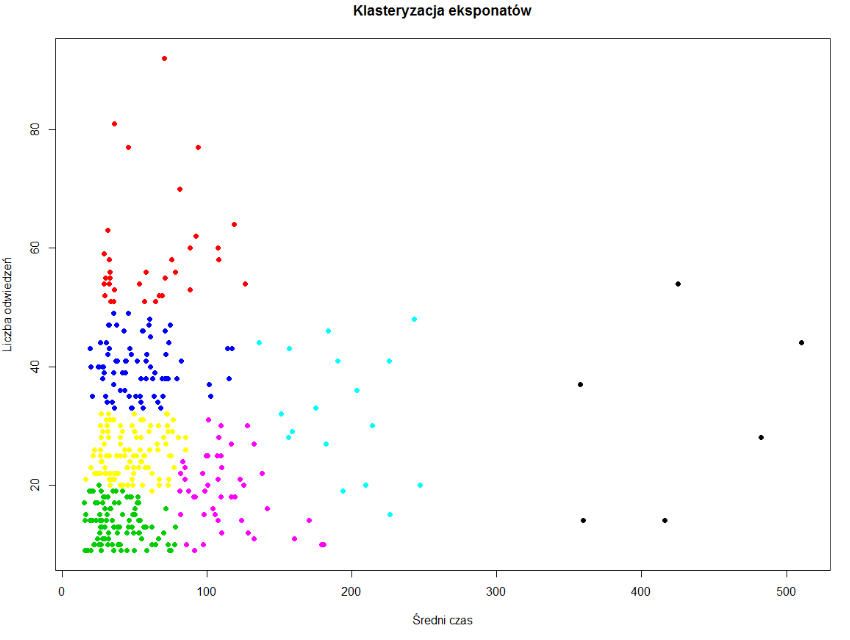
\includegraphics[width=0.48\textwidth]{klasteryzacja_czas_odw.png}
\caption{Klasteryzacja według czasu interakcji i liczby odwiedzeń}
\label{klasteryzacja_czas_odw}
\end{figure}
Sam kształt wykresu pokazuje, że eksponaty zabierające dużo czasu nie znajdowały się wśród najczęściej odwiedzanych. Otrzymane klastry odpowiadają ,,szybkim i bardzo popularnym", ,,szybkim i mało popularnym" i ,,wolnym, a przy okazji przeciętnie popularnym" eksponatom i sytuacjami pomiędzy nimi.

Rysunek \ref{klasteryzacja_czas_zach} ilustruje klasteryzację według czasu interakcji i poziomu eksploracji (w zakresie 1-3, z połączonym wyłącznym dotykaniem i wyłącznym patrzeniem).
\begin{figure}[H]
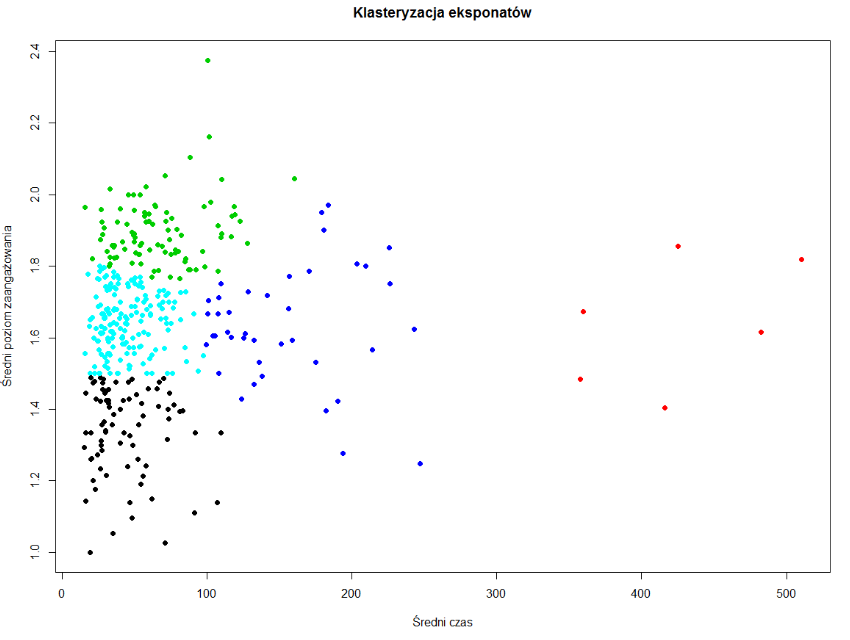
\includegraphics[width=0.48\textwidth]{klasteryzacja_czas_zach.png}
\caption{Klasteryzacja według czasu interakcji i poziomu eksploracji}
\label{klasteryzacja_czas_zach}
\end{figure}
Eksponaty, które nie były eksplorowane (być może dlatego, że nie pozwalały), nie zatrzymywały dzieci na długo. Otrzymane grupy to eksponaty ,,szybkie, mało angażujące", ,,szybkie, dosyć angażujące", ,,szybkie, bardzo angażujące", ,,wolne, dosyć angażujące" i ,,bardzo wolne, dosyć angażujące".

Na wykresie \ref{klasteryzacja_odw_zach} przedstawiona jest ostatnia para -- grupowanie według liczby odwiedzeń i poziomu eksploracji.
\begin{figure}[H]
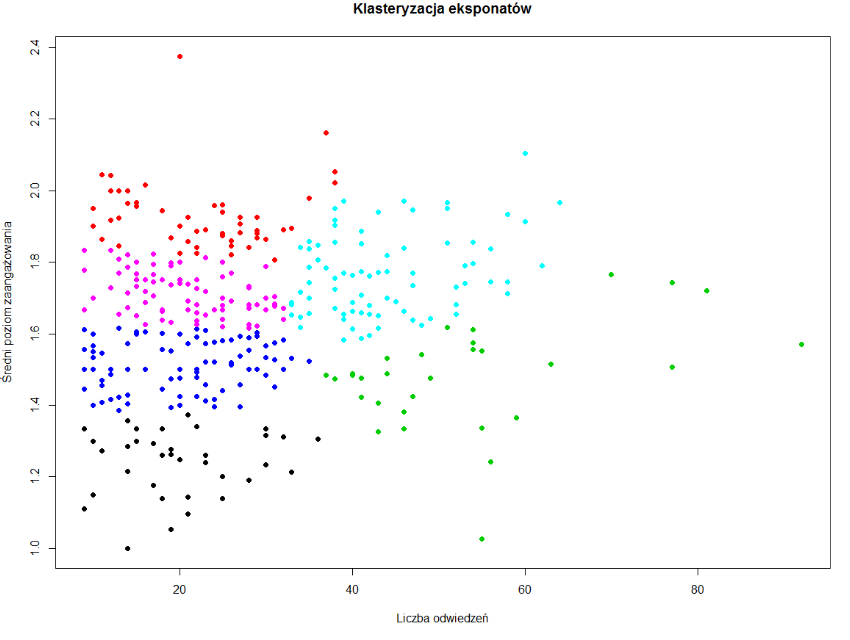
\includegraphics[width=0.48\textwidth]{klasteryzacja_odw_zach.png}
\caption{Klasteryzacja według liczby odwiedzeń i poziomu eksploracji}
\label{klasteryzacja_odw_zach}
\end{figure}
Na wykresie widać, że najczęściej odwiedzane były eksponaty, które były dosyć eksplorowane -- dla porównania istnieje tylko jedna nieeksplorowana wystawa, która uzyskała dużo odwiedzeń -- chodzi tu o \textit{Wahadło Foucault}, które ze swojej natury nie pozwala na nic więcej, niż patrzenie, a jest ulokowane bardzo blisko wejścia. 
Widoczne grupy to eksponaty ,,mało popularne, mało eksplorowane", ,,mało popularne, bardzo eksplorowane", ,,dosyć popularne, bardzo eksplorowane", ,,bardzo popularne, dosyć eksplorowane" i dwie grupy pośrednio eksplorowane i mało popularne.

\section{Wnioski}
\begin{itemize}
\item Dziewczynki mają większą wiedzę o swoich rodzicach -- częściej wiedzą, czy studiowali i gdzie pracują.
\item Liczba książek w domu jest bardzo dobrym predyktorem ocen.
\item Dziewczynki średnio odwiedzają więcej eksponatów, niż chłopcy.
\item Dzieci mają wyższą ocenę z przedmiotu powiązanego z ich wymarzoną pracą, z największą różnicą w przypadku języka polskiego, a najmniejszą w przypadku matematyki.
\item Wykonywanie przez rodziców pracy związanej z danym przedmiotem nieznacznie poprawia rezultaty dzieci, poza matematyką.
\item Dziewczynki częściej trzymają się w stałej grupce.
\item Grupek dziewczęcych, chłopięcych i mieszanych jest mniej więcej tyle samo.
\item Dzieci, które mają gorsze oceny, obejrzały średnio mniej eksponatów.
\item Dzieci z najniższym kapitałem naukowym obejrzały najmniej eksponatów i spędziły przy każdym z nich średnio najmniej czasu.
\item Dzieci z najwyższym kapitałem naukowym rzadziej odwiedzają wielokrotnie ten sam eksponat.
\item Galeria \textit{Lustra} jest specyficzną galerią, w której czas interakcji z eksponatami jest bardzo krótki, mimo wysokiego poziomu eksploracji. Ponadto, tam najczęściej czytane są opisy.
\item Eksponaty bez galerii często zajmują dużo czasu, pozwalają na eksplorację i znacznie częściej dochodzi przy nich do rozmowy z animatorem.
\item Eksponaty, które nie są eksplorowane, zwykle są mniej popularne i interakcja trwa krócej.
\end{itemize}







\end{document}


